\documentclass[]{article}
\usepackage{lmodern}
\usepackage{amssymb,amsmath}
\usepackage{ifxetex,ifluatex}
\usepackage{fixltx2e} % provides \textsubscript
\ifnum 0\ifxetex 1\fi\ifluatex 1\fi=0 % if pdftex
  \usepackage[T1]{fontenc}
  \usepackage[utf8]{inputenc}
\else % if luatex or xelatex
  \ifxetex
    \usepackage{mathspec}
  \else
    \usepackage{fontspec}
  \fi
  \defaultfontfeatures{Ligatures=TeX,Scale=MatchLowercase}
\fi
% use upquote if available, for straight quotes in verbatim environments
\IfFileExists{upquote.sty}{\usepackage{upquote}}{}
% use microtype if available
\IfFileExists{microtype.sty}{%
\usepackage[]{microtype}
\UseMicrotypeSet[protrusion]{basicmath} % disable protrusion for tt fonts
}{}
\PassOptionsToPackage{hyphens}{url} % url is loaded by hyperref
\usepackage[unicode=true]{hyperref}
\hypersetup{
            pdfborder={0 0 0},
            breaklinks=true}
\urlstyle{same}  % don't use monospace font for urls
\usepackage[margin=1in]{geometry}
\usepackage{longtable,booktabs}
% Fix footnotes in tables (requires footnote package)
\IfFileExists{footnote.sty}{\usepackage{footnote}\makesavenoteenv{long table}}{}
\usepackage{graphicx,grffile}
\makeatletter
\def\maxwidth{\ifdim\Gin@nat@width>\linewidth\linewidth\else\Gin@nat@width\fi}
\def\maxheight{\ifdim\Gin@nat@height>\textheight\textheight\else\Gin@nat@height\fi}
\makeatother
% Scale images if necessary, so that they will not overflow the page
% margins by default, and it is still possible to overwrite the defaults
% using explicit options in \includegraphics[width, height, ...]{}
\setkeys{Gin}{width=\maxwidth,height=\maxheight,keepaspectratio}
\IfFileExists{parskip.sty}{%
\usepackage{parskip}
}{% else
\setlength{\parindent}{0pt}
\setlength{\parskip}{6pt plus 2pt minus 1pt}
}
\setlength{\emergencystretch}{3em}  % prevent overfull lines
\providecommand{\tightlist}{%
  \setlength{\itemsep}{0pt}\setlength{\parskip}{0pt}}
\setcounter{secnumdepth}{5}
% Redefines (sub)paragraphs to behave more like sections
\ifx\paragraph\undefined\else
\let\oldparagraph\paragraph
\renewcommand{\paragraph}[1]{\oldparagraph{#1}\mbox{}}
\fi
\ifx\subparagraph\undefined\else
\let\oldsubparagraph\subparagraph
\renewcommand{\subparagraph}[1]{\oldsubparagraph{#1}\mbox{}}
\fi

% set default figure placement to htbp
\makeatletter
\def\fps@figure{htbp}
\makeatother

\usepackage{float}
\usepackage{titling}
\usepackage{caption} 
\usepackage{amsmath}
\usepackage{booktabs}
\captionsetup[table]{skip=8pt}
\usepackage{abstract}
  \renewcommand{\abstractnamefont}{\normalfont\large\bfseries}
\usepackage{booktabs}
\usepackage{longtable}
\usepackage{array}
\usepackage{multirow}
\usepackage{wrapfig}
\usepackage{float}
\usepackage{colortbl}
\usepackage{pdflscape}
\usepackage{tabu}
\usepackage{threeparttable}
\usepackage{threeparttablex}
\usepackage[normalem]{ulem}
\usepackage{makecell}
\usepackage{xcolor}

\author{}
\date{\vspace{-2.5em}}

\begin{document}

\begin{flushleft}
\LARGE{\textbf{Country Level Indicators of Suicide Risk:\\ Data Analysis \& Decision Support for Policy Makers}}\\
\vspace*{2\baselineskip}
\Large{Project Report: Georgia Tech ISyE 6414 - Dr. Yajun Mei}\\
\vspace*{3\baselineskip}
\Large{\textbf{Team Members}}\\
Samuel Garcia\\
Michael Szostak\\ 
Osman Ghandour\\ 
Peter Williams\\
\vspace*{2\baselineskip}
\Large{\textbf{Report Date}}\\
April 21, 2020
\newpage
\end{flushleft}

{
\setcounter{tocdepth}{2}
\tableofcontents
}
\newpage

\begin{abstract}
\bigskip
Relying on open source data from the World Health Organization and other non-governmental bodies, we highlight trends and related to country-level measures of suicide globally. A descriptive model is formulated that identifies a set of meaningful factors and measures that highlights some intuitive relationships between country-level suicide rates and other indicators such as income, alcohol consumption, and the presence of a country level suicide prevention strategy.   

An initial framework for data-driven decision support for policy makers is presented with recommendations including the identification and ongoing monitoring of meaningful factors and measures related to suicide prevention. The hope is that this can provide some introductory guidance for those managing health related planning activities and priorities related to this topic.  

An overview of the sources of data, and process of collection, of data related to suicide at the country level is also described briefly, along with a description of some  ancillary datasets that were employed to augment and enrich insights. The intention of these descriptions is to make further research and data analysis on this topic more accessible to other interested researchers and data analysts in the future.  

\end{abstract}

\section{Research Motivation}\label{research-motivation}

\emph{Peter Sort Bib configuration}

According to the \emph{World Health Organization}, (``Suicide: One
Person Dies Every 40 Seconds'' 2019) one person dies every 40 seconds
from suicide. It is the second leading cause of death among teenagers
and adults aged 15-29 years. Despite the staggering number of suicides
happening worldwide, just 38 governments worldwide have a national
suicide prevention strategy.

Each of these deaths are tragic, and sadly also preventable. For every
suicide, there are many more attempts, and previous suicide attempts are
the single most important predictor or risk factor for future suicide
attempts. (``Suicide: Key Facts'' 2019) The possibility of prevention
and the scale of the problem highlight the need for policy makers, at
the national level, to understand the factors that contribute to suicide
not only in their own nations but also globally.

\subsection{Why is suicide such a complex
problem?}\label{why-is-suicide-such-a-complex-problem}

Suicide is a complex societal problem with multiple social,
psychological, biological, and cultural factors. It is one of the top 20
leading causes of death in the world for all ages (``Alcohol-Related
Risk of Suicidal Ideation, Suicide Attempt, and Completed Suicide: A
Meta-Analysis'' 2015). An estimated one million people die annually from
suicide, i.e., a global mortality rate of 16 per 100,000, or one death
every 40 seconds (``Alcohol-Related Risk of Suicidal Ideation, Suicide
Attempt, and Completed Suicide: A Meta-Analysis'' 2015). Due to the
interactions of so many factors, suicide has no singular cause.

Though it might seem intuitive to categorize suicidal ideation,
attempted suicide, and completed suicide as strictly a psychiatric or
medical issue or a mental illness, not all who commit suicide are
mentally ill. Mental illness is often not clearly distinguishable from
normal distress (``Does Suicide Always Indicate a Mental Illness?''
2009). Stressful experiences, such as exposure to trauma, the death of a
loved one, a job loss, a change in physical health or relationships and
individual characteristics and behaviors are also associated with
suicide (``Suicide Prevention Framework'' 2016).

To underscore the complex nature of the suicide problem, and to show how
causes of suicide can vary between countries, we contrast the situations
in Zimbabwe and Russia. Zimbabwe has suffered endemic poverty,
hyperinflation, and high unemployment for years. On the other hand,
Russia's levels of alcohol consumption are among the highest in the
world. Though their underlying conditions appear to be markedly
different, both nations suffer from high rates of suicide.

\subsection{Examples of the causes of
suicide}\label{examples-of-the-causes-of-suicide}

\subsubsection{Economics - Zimbabwe}\label{economics---zimbabwe}

Political crisis coupled with failed economic policy led to the decline
of Zimbabwe's economic output. Over the past few decades, Zimbabwe's
economic decline has resulted in endemic poverty, hyperinflation, and an
unemployment rate of over 90\% (``The Economic Decline of Zimbabwe''
2009). Zimbabwe's economic woes are often attributed to the policies of
former dictator Robert Mugabe. Post Mugabe, Zimbabwe continues to deal
with debt issues, difficulty attracting foreign investment, and currency
instability.

The WHO estimates that 19 persons per 100k take their own life
deliberately in Zimbabwe per annum (2019). Of the 166 countries in our
study, Zimbabwe ranks 13th in the world for suicides per capita.

\emph{Figure 1: Suicide Rate in Africa (annual persons per 100k
population)}

\begin{center}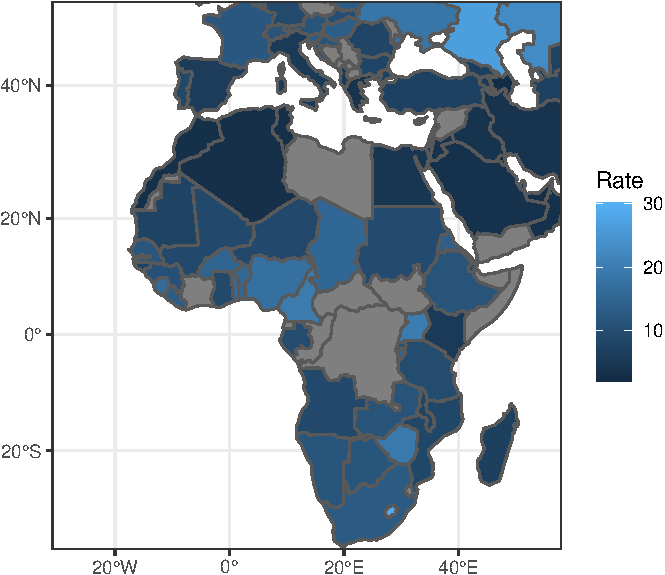
\includegraphics{Project_Report_files/figure-latex/africa_map_plot-1} \end{center}

\emph{Sourced from the World Health Organization report: ``Suicide: Key
Facts, 2019'' and the WorldBank Economic Profile of the Country of
Zimbabwe}

\subsubsection{Alcohol - Russia}\label{alcohol---russia}

Alcohol use disorder (AUD), defined in the WHO's International
Classification of Diseases, is a chronic disease characterized by
compulsive alcohol consumption, loss of control over of alcohol intake,
and negative emotional state when not consuming alcohol. In Russia, the
prevalence of AUD is about 4.7\%, meaning that almost 1-in-20 suffer
from alcohol dependence (``Alcohol Consumption'' 2018). Alcoholism has
been a problem because drinking is not only pervasive, but also a
socially acceptable behavior in Russian society.

The WHO estimates that 27 persons per 100k take their own life
deliberately in Russia per annum (2019). Of the 166 countries in our
study, Russia ranks 3rd in the world for suicides per capita.

\emph{Figure 2: Suicide Rate in Russia (annual persons per 100k
population)}

\begin{center}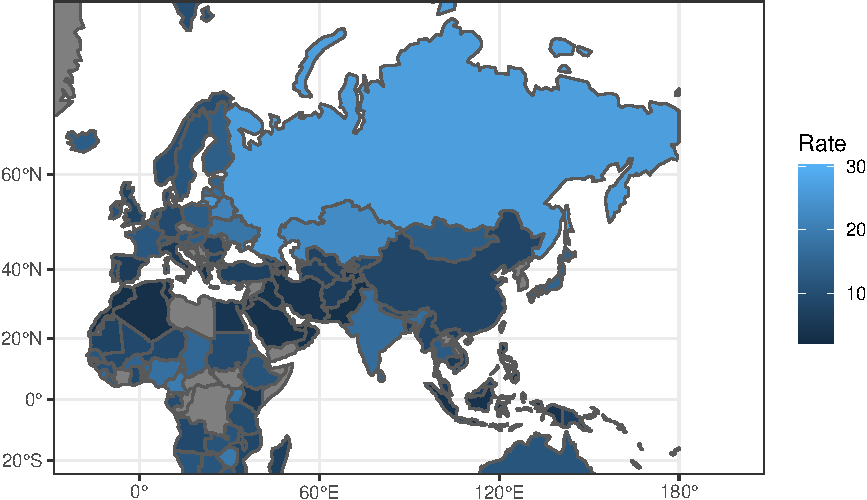
\includegraphics{Project_Report_files/figure-latex/russia_map_plot-1} \end{center}

\emph{Sourced from the World Health Organization report: ``Suicide: Key
Facts, 2019'' and the WorldBank Economic Profile of the Country of
Zimbabwe}

\subsection{Defining the scope of our
research}\label{defining-the-scope-of-our-research}

\section{Variables \& Data Sources}\label{variables-data-sources}

Due to the sheer number of potential factors associated with suicide and
the complex nature of the relationships between them, we wanted to
identify those that were best associated with suicide rates at the
country level. We chose to limit our study to a small set of factors
that could be controlled for and acted upon via policy interventions.

The domains, from which we drew the factors, had to be broad enough to
reasonably represent as many of the potential causes or mitigators of
suicide as possible. Among the domains in consideration were lifestyle,
medical/mental health, economic, and suicide-focused policy.

\textbf{Health Expenditure} and \textbf{GDP per capita} were chosen to
reflect the resources that a country has its disposal to reduce the
suicide rate. \textbf{Liters of Alcohol per capita} was chosen to
account for an aspect of culture (alcohol consumption) that the media
often links to mental health outcomes. The \textbf{presence of a suicide
prevention strategy}, the \textbf{number of psychiatrists}, and the
\textbf{number of mental hospitals} were also chosen to reflect how a
country has deployed its resources to improve mental health outcomes.
The \textbf{female/male labor participation ratio} was also included to
control for trends or changes related to gender labor participation
rates. See the table below for a detailed breakdown.

Due to the sheer number of potential factors associated with suicide and
the complex nature of the relationships between them, we wanted to
identify those that were best associated with suicide rates at the
country level. We chose to limit our study to a small set of factors
that could be controlled for and acted upon via policy interventions.
The domains from which we drew the factors, had to be broad enough to
reasonably represent as many of the potential causes or mitigators of
suicide as possible. Among the domains in consideration were lifestyle,
medical/mental health, economic, and suicide-focused policy. Health
Expenditure and GDP per capita were chosen to reflect the resources that
a country has its disposal to reduce the suicide rate. Liters of Alcohol
per capita was chosen to account for an aspect of culture (alcohol
consumption) that the media often links to mental health outcomes. The
presence of a suicide prevention strategy, the number of psychiatrists,
and the number of mental hospitals were also chosen to reflect how a
country has deployed its resources to improve mental health outcomes.
The female/male labor participation ratio was also included to control
for trends or changes related to gender labor participation rates. See
the table below for a detailed breakdown.

\begin{table}[H]
\centering 
\caption{Data Sources}
\
\begin{tabular}{p{3cm}p{7cm}p{5cm}}  
\hline  
  Input & Data Description  & Source  \\   
\hline 
Current Health Expenditure as a Percentage of GDP & This data provides an indication on the level of resources channeled to health relative to other uses. It shows the importance of the health sector in the whole economy and indicates the societal priority which health is given measured in monetary terms. & World Health Organization [2]  \\   
 \hline 
Labor force participation rate (female-male ratio) & Ratio of female to male of proportion of a country’s working-age population (ages 15 and older) that engages in the labor market, either by working or actively looking for work, expressed as a percentage of the working-age population. & United Nations Development Programme [1] \\   
\hline 
GDP per capita, PPP & Gross Domestic Product converted to international dollars using purchasing power parity (PPP) rates and divided by total population. This data is in terms of PPP in order to account for differences in the cost of living between countries. & World Bank [1] \\
\hline 
Liters of Alcohol per capita &  Total (sum of recorded and unrecorded alcohol) amount of alcohol consumed per person (15 years of age or older) over a calendar year, in liters of pure alcohol, adjusted for tourist consumption. & World Bank [2] \\
\hline 
Suicide Prevention Strategy &  Countries which are known have a stand-alone national suicide prevention strategy are included as 1s, else 0. Note that the plan must be stand-alone, and may not be integrated into another plan, in order to count in the dataset. & World Health Organization [3] \\
\hline
Psychiatrists in mental health, per 100,000 pop. & Number of Psychiatrists working in the mental health sector, per 100,000 population.  & World Health Organization [4]  \\
\hline
Mental hospitals, per 100,000 pop. & Number of hospitals dedicated to mental health per 100,000 population & World Health Organization [5] \\
\hline
\end{tabular} 
\end{table}

\emph{explain (and justify) your proposed methods or models.}

\section{Modeling \& Assumptions}\label{modeling-assumptions}

Our model was developed to infer properties about how a handful of
socioeconomic and cultural indicators impact suicide rates. An important
distinction is that the model is intended to be used for inferential,
rather than predictive purposes. Our objective is to discover
relationships between variables to inform relevant public policy and
future research in the area. The multiple linear regression model was
developed using the following steps: 1. Transformation of Key Outcome
Variable a. Used to make our outcome variable `more normal' b. Helped
characterize relationships between variables in our data c. `Box-Cox'
transformation applied 2. Outlier Removal a. Using regression
diagnostics and visual data exploration we identified unusual data
points b. Removal of outlier was additionally informed by qualitative
reasoning for each country 3. Variable Selection a. Utilized stepwise
regression to identify specific variables for inclusion in our model b.
This `automatic' procedure yielded the set of variables that we would
analyze more closely 4. Final Model Estimation a. Implemented the
``Iteratively Reweighted Least Squares'' approach to estimate model
parameters b. This allowed us to further limit the influence of outliers
on our data

The following variables were selected and included in our model: • Labor
force participation rate, female-male ratio • GDP per capita, PPP •
Liters of Alcohol consumption per capita • Prevalence of a Suicide
Prevention Strategy

Below are the variables that were considered but excluded in step 3 of
the model development: • Current Health Expenditure as a percentage of
GDP • Number of Psychiatrists working in the mental health sector, per
100,000 population • Number of Mental Hospitals, per 100,000 population

In the development of our model, we relied on a few assumptions about
the quality of our data. The first is regarding GDP per capita, which is
assumed to be an appropriate indicator to reflect the wealth of a
country. The second relates to the prevalence of a national suicide
prevention strategy. It is assumed that the presence of such a strategy
is indicative that the country has taken the time to develop a
comprehensive and data driven approach to suicide, based on solid
evidence. We also assume that the liters of alcohol consumed per capita
reflects the tendency for individuals in the given country to consume
excessive amounts of alcohol.

\section{Quantifying Impact of Measures on
Suicide}\label{quantifying-impact-of-measures-on-suicide}

The model described allows the data analyst to describe the
relationships between country-level indicators and measures and suicide
rates globally. Armed with a descriptive model of suicide rates,
decision-makers can quantify the relationships between these measures to
support insight for their health related planning activities. However,
data-driven insights derived from this model and the data sources
highlighted in this report should be considered in context of specific
country-level impacts not considered in this report. As policy makers
infer correlations of country-level measures and indicators with suicide
rates there is a need to continue to engage subject-matter-experts in
the field to draw on their knowledge and experience. Our intention is to
provide some initial context and decision support for policy makers
managing health related planning globally and at the country level, but
the limitations of our research and methodology highlight the ongoing
need for data-driven insights to be utilized in context of other
research available, as well as the domain knowledge of practitioners,
health professionals, scientists, and policy makers among others.

To highlight the need for a holistic approach to gathering data-driven
insights, and incorporating domain knowledge of subject matter experts,
we describe a basic framework for potentially incorporating insights
from our model into a policy decision-making process:

\begin{table}[H]
\centering 
\caption{Framework: Identifying, Describing and Monitoring Country Level Indicators to Support Decision-Making}
\
\begin{tabular}{p{7cm}p{9cm}}  
\hline  
   Area of Focus  & Decision Support  \\   
\hline 
 Identifying \& Quantifying Measures and Indicators of Country Level Suicide Rates &  Using a model to describe the relationships between country-level indicators and suicide rates to help policy makers identify what variables are important and putting context around how to monitor them \\   
 \hline 
Incorporating Domain Knowledge and Expertise of Subject Matter Experts & Allows policy makers to correlate indicators with country-level suicide related outcomes in context of qualitative insights from experts in the field \\   
\hline 
Insight Gathering, Analysis and Support Policy Maker Decisions & Integrating data and insights and providing inital context to help policy makers to frame longer term health planning activities and policies \\
\hline 
\end{tabular} 
\end{table}

In context of providing exemplary decision-support ofr health related
planning activities we discuss some interesting relationships we
identified between country-level suicide rates and the descriptor
variables we selected in the following sections.

\subsection{Quantifying Impact: Income, GDP per
person}\label{quantifying-impact-income-gdp-per-person}

Insights

Our model indicates the presence of a significant relationship between a
measure of income (country-level GDP per person) and suicide~

Countries with lower per person income, tend to have higher incidence of
suicide when controlling for other variables in our model*

Based on our estimates, an approximate 10\% increase in income
corresponds to a 2\% decrease in suicide rate at the country level for
the typical country

\begin{center}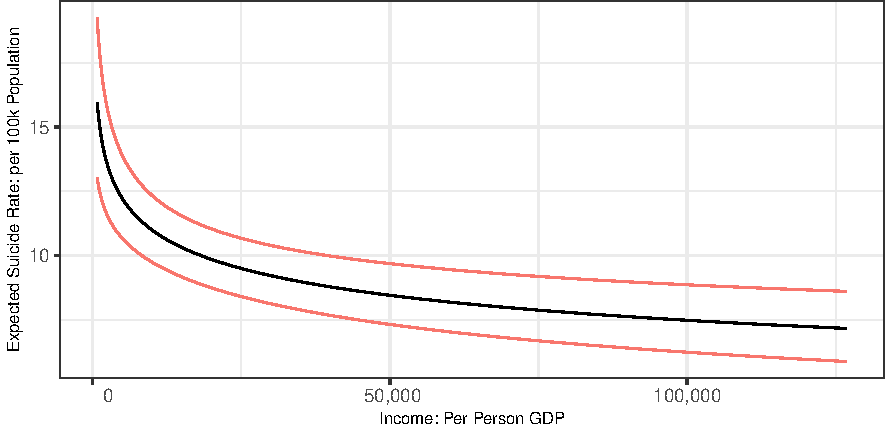
\includegraphics{Project_Report_files/figure-latex/agdp_plot-1} \end{center}

\subsection{Quantifying Impact: Alcohol
Consumption:}\label{quantifying-impact-alcohol-consumption}

Insights

Our model indicates the presence of a significant relationship between a
measure of alcohol consumption (liters per year)

Countries with higher levels of alcohol consumption income, tend to have
higher incidence of suicide when controlling for other variables in our
model*

Based on our estimates, an approximate 4\% increase in alcohol
consumption corresponds to a 2\% increase in suicide rate at the country
level for the typical country (\textgreater{}4 liters per year)

Alcohol consumption was the most impactful and significant indicator of
country-level suicide rate in our analysis

\begin{center}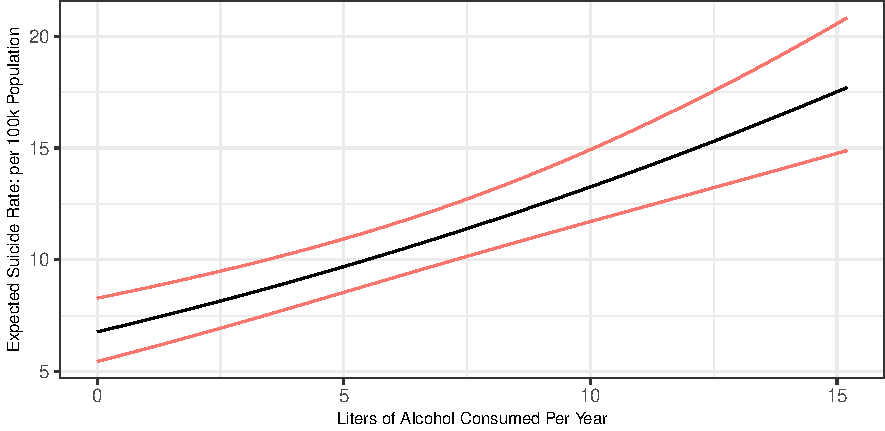
\includegraphics{Project_Report_files/figure-latex/a_alc_plot-1} \end{center}

\subsubsection{Quantifying Impact: The Presence of A National Suicide
Strategy}\label{quantifying-impact-the-presence-of-a-national-suicide-strategy}

Insights

Our model indicates that countries that have put a national suicide
prevention strategy in place, tend to have higher incidence of suicide
rates overall

Based on our estimates, countries that have implemented a suicide
prevention strategy have a 26\% higher incidence of suicide nationally

However, to put this in context, it appears that the institution of a
suicide prevention strategy by countries struggling with suicide
prevention overall, including Guyana, Lithuania, Suriname, Belarus and
South Korea are driving this estimate

\begin{center}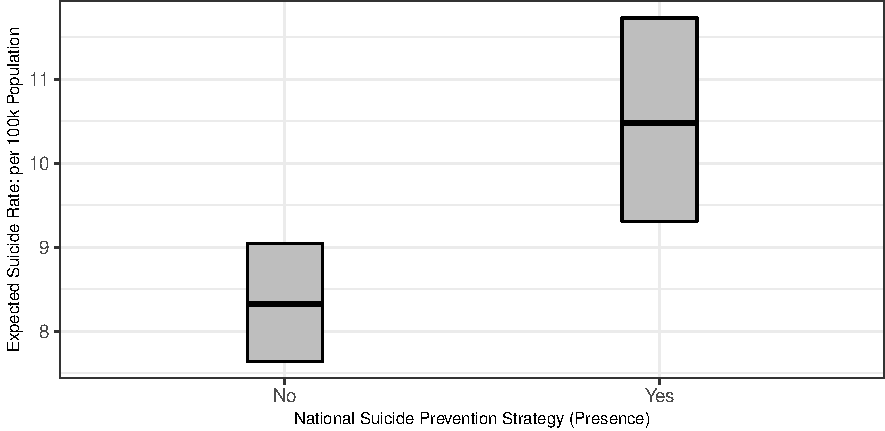
\includegraphics{Project_Report_files/figure-latex/sstrat_plot-1} \end{center}

\section{Recommendations and Decision
Support}\label{recommendations-and-decision-support}

For each of the selected model inputs, there are corresponding
recommendations. The following sections go over each.

\subsection{Suicide Prevention
Strategy}\label{suicide-prevention-strategy}

Even though countries that have put a national suicide prevention
strategy in place, tend to have higher incidence of suicide rates
overall, this is in reaction to their already higher suicide rates in
general. As such it is still advised to have a national strategy to
address suicide. Countries should consider establishing an authoritative
agency, tasked with the continued investigating, formulating, and
implementing of a National Suicide Prevention Strategy. This strategy
can include, but is not limited to, the establishing of a national
suicide crisis line as well as suicide prevention and care services. In
addition, it is best to follow recommended practices set forth by UN
studies which show and help navigate the intersection of biological,
psychological, social, environmental, and cultural factors which
influence suicide, as well as successful policies which countries which
countries which had national suicide prevention programs had
implemented. Devolving countries are recommended to take advantage of
online resources for policy planners the WHO's website MiNDbank for
recommendations on mental health issues (``WHO Mindbank'' 2020). Follow
actions like those below from countries with success in reducing suicide
(``National Suicide Prevention Strategies: Progress, Examples and
Indicators'' 2018): • Reduce access to means and methods of suicide •
View suicide as a psychological mistake • Improve medical, psychological
and psychosocial initiatives • Distribute knowledge about evidence-based
methods for reducing suicide • Raise skill levels among staff and other
key individuals in the care services • Perform ``root cause'' or event
analyses after suicide • Support voluntary organizations

Strategies should not replace existing frameworks already in place in
local government Promote public awareness campaigns highlighting the
prevalence of suicide. By changing public perceptions and reducing the
stigmas associated with seeking help, the rate of suicide can be
reduced.

\subsection{Alcohol Intake}\label{alcohol-intake}

Suicide is a complex societal problem with no singular cause. However,
harmful use of alcohol is among the major risk factors for suicide.
Policy makers should consider implementing measures designed to mitigate
the harmful use of alcohol as a means of reducing the rate of suicide.
According to the WHO, among the policy interventions that have proven
effective at reducing the harmful use of alcohol are varied. One is to
increase the price of alcohol via taxation, which is implemented
successfully in states such as Utah. Another is to enact and enforce
restrictions on alcohol advertising (across multiple types of media),
out of sight out of mind. And finally, enact and enforce restrictions on
the physical availability of retailed alcohol (via reduced hours of
sale), for example many ``dry states'' do not serve alcohol on Sundays
(``Global Status Report on Alcohol and Health 2018'' 2018). It is not
recommended to remove access to alcohol completely, as seen in the
disastrous US history lesson in the prohibition era. The increased
violence may not have been worth the decrease in suicide (``The Effects
of War and Alcohol Consumption Patterns on Suicide: United States,
1910-1933'' 1989).

\subsection{GDP Per Capita}\label{gdp-per-capita}

There is a negative correlation between GDP per capita and suicide
rates. While it is unknown why this is, we believe that money should be
spent to uncover more about the relationship between income and suicide.
An analysis on income of specific income groups would shed more light as
to whether low income correlates to higher suicide or not. As such it is
recommended Invest in research to better understand potential
relationships between income instability, income protection and suicide
at the individual level. In addition, governments should pursue measures
aimed at poverty reduction and unemployment benefits to support economic
well-being.

Even though countries that have put a national suicide prevention
strategy in place, tend to have higher incidence of suicide rates
overall, this is in reaction to their already higher suicide rates in
general. As such it is still advised to have a national strategy to
address suicide. Countries should consider establishing an authoritative
agency, tasked with the continued investigating, formulating, and
implementing of a National Suicide Prevention Strategy. This strategy
can include, but is not limited to, the establishing of a national
suicide crisis line as well as suicide prevention and care services. In
addition, it is best to follow recommended practices set forth by UN
studies which show and help navigate the intersection of biological,
psychological, social, environmental, and cultural factors which
influence suicide, as well as successful policies which countries which
countries which had national suicide prevention programs had
implemented. Devolving countries are recommended to take advantage of
online resources for policy planners the WHO's website MiNDbank for
recommendations on mental health issues {[}1{]}. Follow actions like
those below from countries with success in reducing suicide {[}2{]}: •
Reduce access to means and methods of suicide • View suicide as a
psychological mistake • Improve medical, psychological and psychosocial
initiatives • Distribute knowledge about evidence-based methods for
reducing suicide • Raise skill levels among staff and other key
individuals in the care services • Perform ``root cause'' or event
analyses after suicide • Support voluntary organizations Strategies
should not replace existing frameworks already in place in local
government Promote public awareness campaigns highlighting the
prevalence of suicide. By changing public perceptions and reducing the
stigmas associated with seeking help, the rate of suicide can be
reduced. {[}1{]} \url{https://www.who.int/mental_health/mindbank/en/}
{[}2{]} \url{https://apps.who.int/iris/rest/bitstreams/1174021/retrieve}

\subsection{Alcohol Intake}\label{alcohol-intake-1}

Suicide is a complex societal problem with no singular cause. However,
harmful use of alcohol is among the major risk factors for suicide.
Policy makers should consider implementing measures designed to mitigate
the harmful use of alcohol as a means of reducing the rate of suicide.
According to the WHO, among the policy interventions that have proven
effective at reducing the harmful use of alcohol are varied. One is to
increase the price of alcohol via taxation, which is implemented
successfully in states such as Utah. Another is to enact and enforce
restrictions on alcohol advertising (across multiple types of media),
out of sight out of mind. And finally, enact and enforce restrictions on
the physical availability of retailed alcohol (via reduced hours of
sale), for example many ``dry states'' do not serve alcohol on Sundays.
{[}1{]} It is not recommended to remove access to alcohol completely as
seen in the disastrous US history lesion in the prohibition era. The
increased violence may not have been worth the decrease in suicide.
{[}2{]}{[}1{]} ``WHO \textbar{} Global status report on alcohol and
health 2018 - World \ldots{}.'' 21 Sep. 2018,
\url{https://www.who.int/substance_abuse/publications/global_alcohol_report/en/}.
Accessed 5 Apr. 2020. {[}2{]}
\url{https://academic.oup.com/sf/article-abstract/68/2/513/1927193}

\subsection{Income \& GDP Per Capita}\label{income-gdp-per-capita}

There is a negative correlation between GDP per capita and suicide
rates. While it is unknown why this is, we believe that money should be
spent to uncover more about the relationship between income and suicide.
An analysis on income of specific income groups would shed more light as
to whether low income correlates to higher suicide or not. As such it is
recommended Invest in research to better understand potential
relationships between income instability, income protection and suicide
at the individual level. In addition, governments should pursue measures
aimed at poverty reduction and unemployment benefits to support economic
well-being.

\section{Research Limitations}\label{research-limitations}

In any study there are limitations on what is considered in analysis. We
only considered a limited set of inputs and analysis measures in the
allotted time and would perform more had there been more. A breakdown of
the research limitations of scope, what was considered, and methodology,
how it was analyzed, are described below.

\subsection{Scope}\label{scope}

There were issues with some of our inputs, but when drilling down to
just the inputs used in the model, we can see room for improvement in
data quality. When we used GDP per Capita as a proxy for income, other
measures such as country-level median income should have been considered
in the future. This would have given a non-uniform distribution of
wealth in the country rather than a uniform distribution which is not
the case with income inequality. When measuring the liters of alcohol
consumed, we assumed a uniform consumption country-wide consumption
rate. This doesn't consider incidence of substance abuse. For Suicide
Policy (NSPS), the effectiveness of organizational response hard per
country is hard to gauge since local response vs federal not accounted
for in measurement. We did not consider local/cultural/interactional
measures making it difficult to make country-specific inferences in some
cases.

\subsection{Methodology}\label{methodology}

For our analysis we chose to use a country level scope, however this
cannot drill down to local or individual level, essentially limiting our
level of fidelity of reflecting on reality. For each country we only
used one year, as such our model assumes effects of each input are fixed
rather than temporally differing. When considering our inputs, we cannot
completely untangle the effect of variable interactions between another.
Higher level interactions and additional factors which may influence
suicide rates could be considered in the future. Finally, model
formulation limited our analysis strength. We chose to use multiple
linear regression for inferential and descriptive reasons, but more
complicated / non-linear relationships could be characterized better
with more complex approaches.

\newpage 

There were issues with some of our inputs, but when drilling down to
just the inputs used in the model, we can see room for improvement in
data quality. When we used GDP per Capita as a proxy for income, other
measures such as country-level median income should have been considered
in the future. This would have given a non-uniform distribution of
wealth in the country rather than a uniform distribution which is not
the case with income inequality. When measuring the liters of alcohol
consumed, we assumed a uniform consumption country-wide consumption
rate. This doesn't consider incidence of substance abuse. For Suicide
Policy (NSPS), the effectiveness of organizational response hard per
country is hard to gauge since local response vs federal not accounted
for in measurement. We did not consider local/cultural/interactional
measures making it difficult to make country-specific inferences in some
cases.

\subsection{Methodology}\label{methodology-1}

For our analysis we chose to use a country level scope, however this
cannot drill down to local or individual level, essentially limiting our
level of fidelity of reflecting on reality. For each country we only
used one year, as such our model assumes effects of each input are fixed
rather than temporally differing. When considering our inputs, we cannot
completely untangle the effect of variable interactions between another.
Higher level interactions and additional factors which may influence
suicide rates could be considered in the future. Finally, model
formulation limited our analysis strength. We chose to use multiple
linear regression for inferential and descriptive reasons, but more
complicated non-linear relationships could be characterized better with
more complex approaches.

\section{Appendix \& References}\label{appendix-references}

\emph{This section only includes needed documents to support the
presentation in the report. Feel free to divide it into several
subsections if necessary. Do NOT dump all computer outputs unor-ganized
here}

\subsection{Model Final Specification}\label{model-final-specification}

\[
\begin{aligned}
& Y_i = \beta_0 + \beta_1 x_{1i} + \beta_2 x_{2i} + \beta_3 x_{3i} + \beta_4 x_{4i}  + \epsilon_i,\ \text{where we assumed, } \epsilon_i \sim \mathbb{N}(0,\sigma_{Y}^2) \\
&\\
&\text{for } i = 1,...,n \ \text{country level measures, where} \\
& \\
& Y_i \ \ : \text{The estimated national suicide rate (per 100k population) for the} i^{\text{th}} \text{ country.(Box-cox transformed $\lambda = 0.4$)} \\
& x_{1i}\ : \text{The estimated national labor participation rate (percentage) for the } i^{\text{th}} \text{ country.}\\
& x_{2i}\ : \text{The log-transformed estimated per-person gross domestic product (GDP) (income) for the } i^{\text{th}} \text{ country.}\\
& x_{3i}\ : \text{An estimate of the national per-person average of liters of alcohol consumed annually for the } i^{\text{th}} \text{ country.}\\
& x_{4i}\ : \text{A binary indicator of the 'presence of a national suicide prevention strategy' in 2019 for the } i^{\text{th}} \text{ country.}\\
& \\
& \text{This yields fitted regression model: } \\
& \\
& \hat{Y_i} = \hat{\beta_0} + \hat{\beta_1} x_{1i} + \hat{\beta_2} x_{2i} + \hat{\beta_3} x_{3i} + \hat{\beta_4} x_{4i} \\
& \\
& \text{where, } \\
& \\
& \hat{\beta_0},\ \hat{\beta_1},\ \hat{\beta_2},\ \hat{\beta_3}, \ \text{and } \hat{\beta_4} \text{ were estimated by the method of iterative re-weighted least squares.} \\
\end{aligned}
\]

\subsection{Model Summary Statistics}\label{model-summary-statistics}

\begin{table}[H] \centering 
  \caption {Regression Model Summary} 
  \label{tab:title} 
\begin{tabular}{@{\extracolsep{5pt}}lc} 
\\[-1.8ex]\hline 
\hline \\[-1.8ex] 
 & \multicolumn{1}{c}{\textit{Dependent variable:}} \\ 
\cline{2-2} 
\\[-1.8ex] & Suicide Rate (Box-Cox Transformed $\lambda = 0.4$) \\ 
\hline \\[-1.8ex] 
 Income (pp GDP) - Log Transformed & $-$0.404$^{***}$ \\ 
  & (0.080) \\ 
  & \\ 
Liters of Alcohol Consumed & 0.166$^{***}$ \\ 
  & (0.026) \\ 
  & \\ 
Suicide Prevention Strategy (Binary) & 0.562$^{***}$ \\ 
  & (0.185) \\ 
  & \\ 
Labor Participation Rate & 1.031$^{**}$ \\ 
  & (0.472) \\ 
  & \\ 
 Constant & 5.420$^{***}$ \\ 
  & (0.828) \\ 
  & \\ 
\hline \\[-1.8ex] 
Observations & 162 \\ 
R$^{2}$ & 0.412 \\ 
Adjusted R$^{2}$ & 0.397 \\ 
Residual Std. Error & 1.272 (df = 157) \\ 
F Statistic & 27.475$^{***}$ (df = 4; 157) \\ 
\hline 
\hline \\[-1.8ex] 
\textit{Note:}  & \multicolumn{1}{r}{$^{*}$p$<$0.1; $^{**}$p$<$0.05; $^{***}$p$<$0.01} \\ 
\end{tabular} 
\end{table}

\newpage

\subsection{Additional Details: Modeling
Approach}\label{additional-details-modeling-approach}

\subsection{Initial Model Choice and
Transformation}\label{initial-model-choice-and-transformation}

We developed a multiple linear regression model to infer properties
about how a handful of socioeconomic and cultural indicators impact
suicide rates. Initial Model, First, we analyzed the diagnostic plots to
understand if our model appropriately fits the data that we have. A
major red flag here was the Normal Q-Q plot, which shows if residuals
are normally distributed. The residuals deviate from the reference line
at the higher quintiles. In order to correct for this, our next step was
to try a Box Cox transformation on Y. Below is the log-likelihood plot
to determine the lambda value for the Box Cox transformation. A lambda
value of 0.4 was chosen.

We also applied log transformation to the variable GDP per capita to
better represent the relationship between this variable and the outcome
variable based on visual data exploration and resulting effect .

\subsection{Outlier Removal Decisions}\label{outlier-removal-decisions}

\emph{Create table here??}

The next step in model development was to remove outliers. Points 12,
65, and 88 were identified as outliers on the Residuals vs Fitted,
Scale-Location, and Normal Q-Q plots.

In addition, point 79 was identified as an outlier that should be
removed, as it had very high leverage in the model.

Points 12, 65, 79, and 88 were removed from the dataset. It is important
to note that each of these points also had country specific reasons for
being excluded:

After the removal of outliers, we implemented a backwards stepwise
algorithm based on AIC to remove variables that were redundant or
unnecessary in the model.

\subsection{Stepwise Variable Selection
Approach}\label{stepwise-variable-selection-approach}

We implemented a backwards stepwise algorithm based on AIC to remove
variables based on the AIC criterion, the results and variable inclusion
decisions are detailed below:

\begin{table}[H]
\centering 
\caption{Variable Selection Details: Backwards Stepwise Regression (AIC Criterion)}
\
\begin{tabular}{p{5cm}p{4cm}}  
\hline  
Variable & Model Inclusion Result \\  
\hline
GDP per capita, PPP & Included \\
\hline 
Prevalence of a national suicide prevention strategy & Included \\
\hline 
Liters of alcohol consumption per capita & Included \\
\hline 
Male to Female ratio of the labor participation rate & Included \\
\hline
Health Expenditure as a percentage of GDP & Removed \\
 \hline 
Psychiatrists working in mental health sector (per 100 000 population) & Removed \\   
\hline 
Mental hospitals (per 100 000 population) &  Removed \\
\hline 
\end{tabular} 
\end{table}

The final step in preparing the model was to implement the iteratively
weighted least squares algorithm to properly weight each instance in our
data. This was more effort to mitigate the effect of outliers on our
model. We performed 10 iterations of this algorithm.

\section*{References}\label{references}
\addcontentsline{toc}{section}{References}

\hypertarget{refs}{}
\hypertarget{ref-russia2018}{}
``Alcohol Consumption.'' 2018.
\url{https://ourworldindata.org/alcohol-consumption}.

\hypertarget{ref-ideation2015}{}
``Alcohol-Related Risk of Suicidal Ideation, Suicide Attempt, and
Completed Suicide: A Meta-Analysis.'' 2015.
\url{https://www.ncbi.nlm.nih.gov/pmc/articles/PMC4439031/}.

\hypertarget{ref-mental2009}{}
``Does Suicide Always Indicate a Mental Illness?'' 2009.
\url{https://www.ncbi.nlm.nih.gov/pmc/articles/PMC4222167/}.

\hypertarget{ref-alcoholreport}{}
``Global Status Report on Alcohol and Health 2018.'' 2018.
\href{\%20https://www.who.int/substance_abuse/publications/global_alcohol_report/en/}{https://www.who.int/substance\_abuse/publications/global\_alcohol\_report/en/}.

\hypertarget{ref-strategy}{}
``National Suicide Prevention Strategies: Progress, Examples and
Indicators.'' 2018.
\href{\%20https://apps.who.int/iris/handle/10665/279765}{https://apps.who.int/iris/handle/10665/279765}.

\hypertarget{ref-framework2016}{}
``Suicide Prevention Framework.'' 2016.
\url{https://www.canada.ca/en/public-health/services/publications/healthy-living/suicide-prevention-framework.html}.

\hypertarget{ref-stats2019}{}
``Suicide: Key Facts.'' 2019.
\url{https://www.who.int/news-room/fact-sheets/detail/suicide}.

\hypertarget{ref-who2019}{}
``Suicide: One Person Dies Every 40 Seconds.'' 2019.
\url{https://www.who.int/news-room/detail/09-09-2019-suicide-one-person-dies-every-40-seconds}.

\hypertarget{ref-zimbabwe2009}{}
``The Economic Decline of Zimbabwe.'' 2009.
\url{https://cupola.gettysburg.edu/cgi/viewcontent.cgi?article=1021\&context=ger}.

\hypertarget{ref-prohibition}{}
``The Effects of War and Alcohol Consumption Patterns on Suicide: United
States, 1910-1933.'' 1989.
\href{\%20https://apps.who.int/iris/rest/bitstreams/1174021/retrieve}{https://apps.who.int/iris/rest/bitstreams/1174021/retrieve}.

\hypertarget{ref-mindbank}{}
``WHO Mindbank.'' 2020.
\url{https://www.who.int/mental_health/mindbank/en/}.

\end{document}
